\documentclass[border=3mm]{article}

\usepackage{pgfplots}

% Unit circle plot style
\pgfplotsset{unit circle/.style={width=4cm,height=4cm,axis lines=middle,xtick=\empty,ytick=\empty,axis equal,enlargelimits,xmax=1.4,ymax=1.4,xmin=-1.4,ymin=-1.4,domain=0:pi/2}}

\begin{document}
	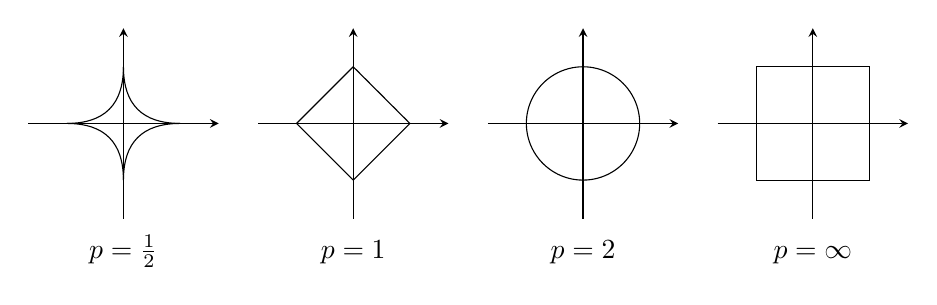
\begin{tikzpicture}
		\coordinate (prev); % Store previous plot position
		\foreach \p / \t in {4/\frac{1}{2}, 2/1, 1/2, 0.0001/\infty} { % Loop through the plots to draw
			% \p is the exponent in the function to plot
			% \t is the p parameter to print
			\begin{axis}[at={(prev)},unit circle,anchor=west]
				\foreach \ss in {1,-1} {
					\foreach \cs in {1,-1} {
						\addplot[] ({\cs*(cos(deg(x)))^\p},{\ss*(sin(deg(x))^\p});
					}
				}
			\end{axis}
			\node[below=0.5cm, anchor=base] at (current axis.south) {$p=\t$}; % Print p
			\coordinate[right=0.5cm] (prev) at (current axis.east) ; % Set position for next plot
		}
	\end{tikzpicture}
	
	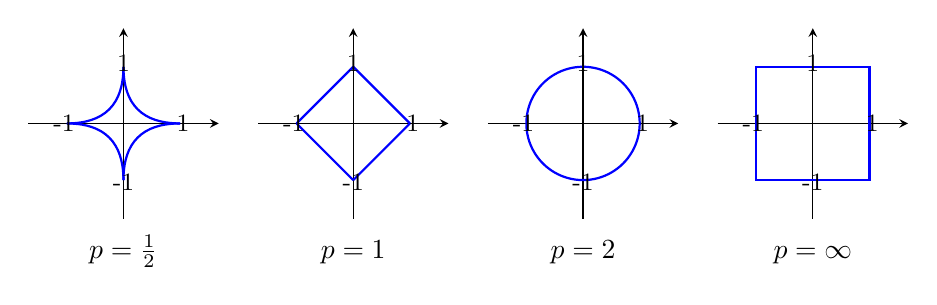
\begin{tikzpicture}
		\coordinate (prev); % Store previous plot position
		\foreach \p / \t in {4/\frac{1}{2}, 2/1, 1/2, 0.0001/\infty} { % Loop through plots
			\begin{axis}[at={(prev)},unit circle,anchor=west]
				% Draw unit circle (dashed gray)
				%\addplot [gray, dashed, domain=0:360, samples=200] ({cos(x)}, {sin(x)});
				
				% Plot the normed shape
				\foreach \ss in {1,-1} {
					\foreach \cs in {1,-1} {
						\addplot [blue, thick] 
						({\cs*(cos(deg(x)))^\p},{\ss*(sin(deg(x)))^\p});
					}
				}
				
				% Add +1 and -1 labels
				\node[font=\small] at (axis cs:1.05,0) {1};
				\node[font=\small] at (axis cs:-1.05,0) {-1};
				\node[font=\small] at (axis cs:0,1.05) {1};
				\node[font=\small] at (axis cs:0,-1.05) {-1};
			\end{axis}
			\node[below=0.5cm, anchor=base] at (current axis.south) {$p=\t$}; % Label under plot
			\coordinate[right=0.5cm] (prev) at (current axis.east); % Move to next position
		}
	\end{tikzpicture}
	
	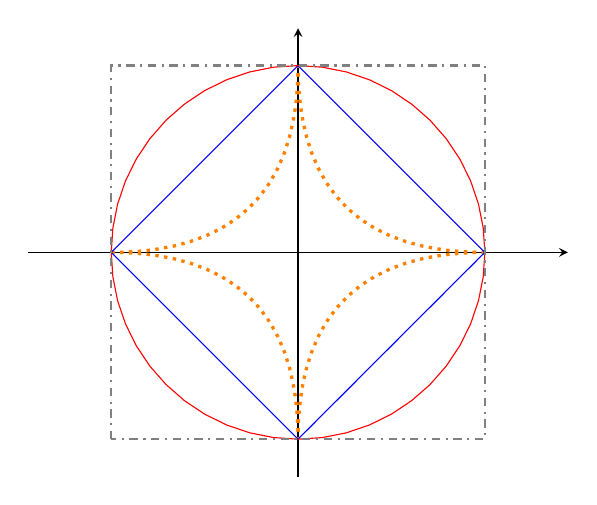
\begin{tikzpicture}
		\begin{axis}[axis lines=middle,xtick=\empty,ytick=\empty,axis equal,enlargelimits,xmax=1,ymax=1,xmin=-1,ymin=-1]
			%p=0.5
			\begin{scope}[very thick,dotted,orange,domain=0:pi,samples=50]
				\addplot[] ({(cos(deg(x)))^(4},{ (sin(deg(x))^(4});
				\addplot[] ({(cos(deg(x)))^(4},{ -(sin(deg(x))^(4});
				\addplot[] ({-(cos(deg(x)))^(4},{ (sin(deg(x))^(4});
				\addplot[] ({-(cos(deg(x)))^(4},{-(sin(deg(x))^(4});
			\end{scope}
			%p=1
			\addplot[blue,domain=0:pi] ({(cos(deg(x)))^2},{(sin(deg(x))^2});
			\addplot[blue,domain=0:pi] ({(cos(deg(x)))^2},{-(sin(deg(x))^2});
			\addplot[blue,domain=0:pi] ({-(cos(deg(x)))^2},{(sin(deg(x))^2});
			\addplot[blue,domain=0:pi] ({-(cos(deg(x)))^2},{-(sin(deg(x))^2});
			%p=2
			\addplot[red,domain=-pi:0] ({(cos(deg(x)))},{(sin(deg(x))});
			\addplot[red,domain=0:pi] ({(cos(deg(x)))},{(sin(deg(x))});
			%p=inf
			\draw[thick,dashdotted,gray] (axis cs:-1,-1) rectangle (axis cs:1,1);
		\end{axis}
	\end{tikzpicture}
	
	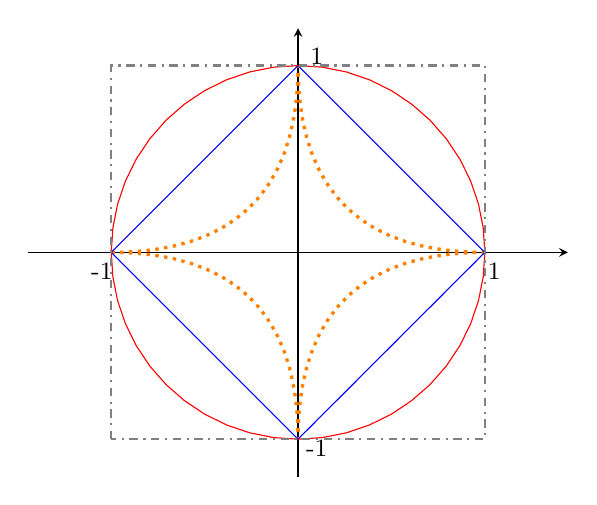
\begin{tikzpicture}
		\begin{axis}[axis lines=middle,xtick=\empty,ytick=\empty,axis equal,enlargelimits,xmax=1,ymax=1,xmin=-1,ymin=-1]
			%p=0.5
			\begin{scope}[very thick,dotted,orange,domain=0:pi,samples=50]
				\addplot[] ({(cos(deg(x)))^(4},{ (sin(deg(x))^(4});
				\addplot[] ({(cos(deg(x)))^(4},{ -(sin(deg(x))^(4});
				\addplot[] ({-(cos(deg(x)))^(4},{ (sin(deg(x))^(4});
				\addplot[] ({-(cos(deg(x)))^(4},{-(sin(deg(x))^(4});
			\end{scope}
			%p=1
			\addplot[blue,domain=0:pi] ({(cos(deg(x)))^2},{(sin(deg(x))^2});
			\addplot[blue,domain=0:pi] ({(cos(deg(x)))^2},{-(sin(deg(x))^2});
			\addplot[blue,domain=0:pi] ({-(cos(deg(x)))^2},{(sin(deg(x))^2});
			\addplot[blue,domain=0:pi] ({-(cos(deg(x)))^2},{-(sin(deg(x))^2});
			%p=2
			\addplot[red,domain=-pi:0] ({(cos(deg(x)))},{(sin(deg(x))});
			\addplot[red,domain=0:pi] ({(cos(deg(x)))},{(sin(deg(x))});
			%p=inf
			\draw[thick,dashdotted,gray] (axis cs:-1,-1) rectangle (axis cs:1,1);
		
			% Add +1 and -1 labels
			\node[font=\small] at (axis cs:1.05,-0.1) {1};
			\node[font=\small] at (axis cs:-1.05,-0.1) {-1};
			\node[font=\small] at (axis cs:0.1,1.05) {1};
			\node[font=\small] at (axis cs:0.1,-1.05) {-1};		
		
		\end{axis}
	\end{tikzpicture}
	    
	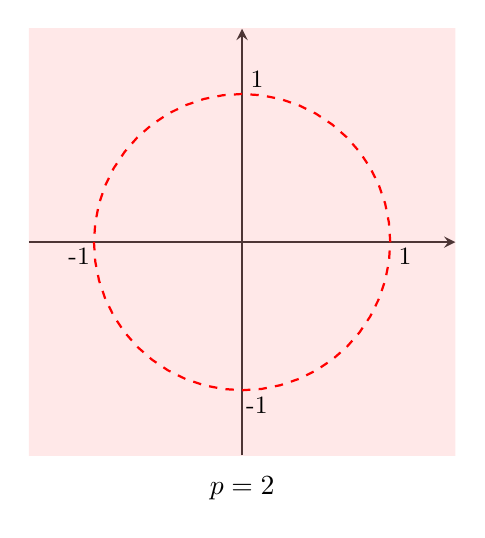
\begin{tikzpicture}
		\begin{axis}[
			width=7cm, height=7cm,
			axis lines=middle,
			xtick=\empty, ytick=\empty,
			axis equal,
			enlargelimits,
			xmin=-1.2, xmax=1.2,
			ymin=-1.2, ymax=1.2,
			thick,
			domain=0:90
			]
			
			\draw [fill = red!30, opacity=0.3, draw=none]  (axis cs:0,0) circle[radius=100];
			
			%p=2
			\addplot[red,domain=-pi:0,  thick, dashed] ({(cos(deg(x)))},{(sin(deg(x))});
			\addplot[red,domain=0:pi,  thick, dashed] ({(cos(deg(x)))},{(sin(deg(x))});
			
			
			% Add +1 and -1 labels
			\node[font=\small] at (axis cs:1.1,-0.1) {1};
			\node[font=\small] at (axis cs:-1.1,-0.1) {-1};
			\node[font=\small] at (axis cs:0.1,1.1) {1};
			\node[font=\small] at (axis cs:0.1,-1.1) {-1};		
			
		\end{axis}
		\node[below=0.5cm, anchor=base] at (current axis.south) {$p=2$}; % Print p
	\end{tikzpicture}
 
 
	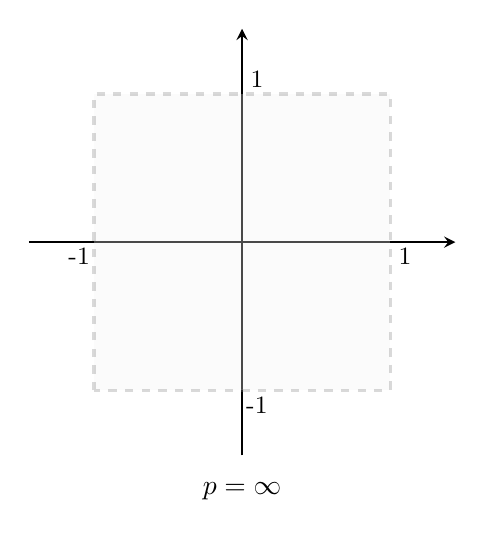
\begin{tikzpicture}
		\begin{axis}[
			width=7cm, height=7cm,
			axis lines=middle,
			xtick=\empty, ytick=\empty,
			axis equal,
			enlargelimits,
			xmin=-1.2, xmax=1.2,
			ymin=-1.2, ymax=1.2,
			thick,
			domain=0:90
			]
			
			%p=inf
			\draw[very thick, dashed, gray, fill=gray!10, opacity=0.3,] (axis cs:-1,-1) rectangle (axis cs:1,1);
			
			% Add +1 and -1 labels
			\node[font=\small] at (axis cs:1.1,-0.1) {1};
			\node[font=\small] at (axis cs:-1.1,-0.1) {-1};
			\node[font=\small] at (axis cs:0.1,1.1) {1};
			\node[font=\small] at (axis cs:0.1,-1.1) {-1};		
			
		\end{axis}
		\node[below=0.5cm, anchor=base] at (current axis.south) {$p=\infty$}; % Print p
	\end{tikzpicture}
  
	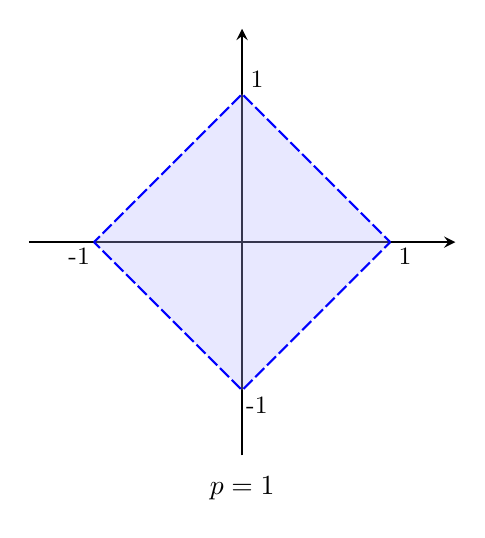
\begin{tikzpicture}
		\begin{axis}[
			width=7cm, height=7cm,
			axis lines=middle,
			xtick=\empty, ytick=\empty,
			axis equal,
			enlargelimits,
			xmin=-1.2, xmax=1.2,
			ymin=-1.2, ymax=1.2,
			thick,
			domain=0:90
			]
			
			\addplot  [fill=blue!30, opacity=0.3, draw=none] coordinates { (0,1) (-1,0) (0,-1) (1,0)}
			--cycle;
			
			
			\foreach \sx in {1,-1} {
				\foreach \sy in {1,-1} {
					\addplot[blue, domain=0:pi,  thick, dashed]
					({\sx*(cos(deg(x)))^2}, {\sy*(sin(deg(x)))^2});
				}
			}
			
			% Add +1 and -1 labels
			\node[font=\small] at (axis cs:1.1,-0.1) {1};
			\node[font=\small] at (axis cs:-1.1,-0.1) {-1};
			\node[font=\small] at (axis cs:0.1,1.1) {1};
			\node[font=\small] at (axis cs:0.1,-1.1) {-1};		
			
		\end{axis}
		\node[below=0.5cm, anchor=base] at (current axis.south) {$p=1$}; % Print p
	\end{tikzpicture}
 
 
 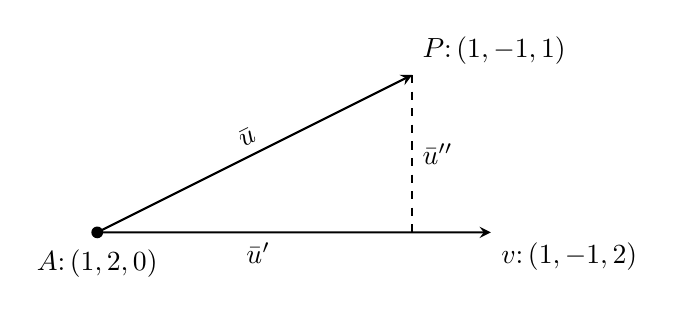
\begin{tikzpicture}[x={(0,0)},y={(-1cm,-4cm/3)},z={(1cm,-2cm)},thick,auto]
 	\draw[-stealth]  (1,2,0) 
 	node[circle,fill,inner sep=1.5pt,label=below:{$A\colon(1,2,0)$}] (A){} 
 	-- node[sloped] {$\bar u$} 
 	(1,-1,1) coordinate[label=above right:{$P\colon(1,-1,1)$}](P);
 	\draw[dashed] (P) -- node{$\bar u''$} (P|-A);
 	\path (A)  -- node[swap]{$\bar u'$} (P|-A);
 	\draw[-stealth] (1,2,0) -- (1,-1,2)
 	coordinate[label=below right:{$v\colon(1,-1,2)$}](v);
 \end{tikzpicture}


%\tikzset{every picture/.style={line width=0.75pt}} %set default line width to 0.75pt        

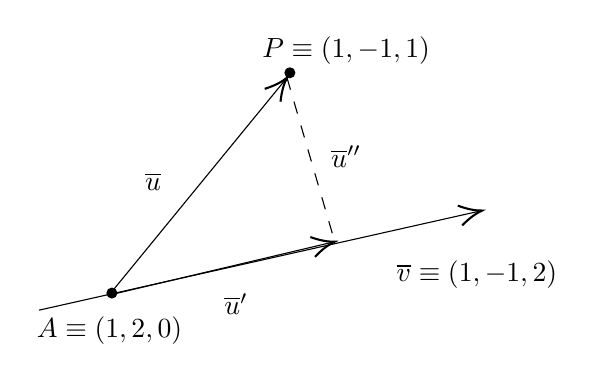
\begin{tikzpicture}[x=0.75pt,y=0.75pt,yscale=-1,xscale=1]
	%uncomment if require: \path (0,300); %set diagram left start at 0, and has height of 300
	
	%Straight Lines [id:da6137486785624535] 
	\draw    (119,195) -- (330.55,147.44) ;
	\draw [shift={(332.5,147)}, rotate = 527.3299999999999] [color={rgb, 255:red, 0; green, 0; blue, 0 }  ][line width=0.75]    (10.93,-4.9) .. controls (6.95,-2.3) and (3.31,-0.67) .. (0,0) .. controls (3.31,0.67) and (6.95,2.3) .. (10.93,4.9)   ;
	
	%Straight Lines [id:da46366121878923283] 
	\draw    (152.75,187.75) -- (237.23,84.55) ;
	\draw [shift={(238.5,83)}, rotate = 489.3] [color={rgb, 255:red, 0; green, 0; blue, 0 }  ][line width=0.75]    (10.93,-4.9) .. controls (6.95,-2.3) and (3.31,-0.67) .. (0,0) .. controls (3.31,0.67) and (6.95,2.3) .. (10.93,4.9)   ;
	
	%Straight Lines [id:da030080067558663437] 
	\draw  [dash pattern={on 4.5pt off 4.5pt}]  (238.5,83) -- (261.5,162) ;
	
	
	%Straight Lines [id:da5041853499131848] 
	\draw    (152.75,187.75) -- (259.55,162.46) ;
	\draw [shift={(261.5,162)}, rotate = 526.6800000000001] [color={rgb, 255:red, 0; green, 0; blue, 0 }  ][line width=0.75]    (10.93,-4.9) .. controls (6.95,-2.3) and (3.31,-0.67) .. (0,0) .. controls (3.31,0.67) and (6.95,2.3) .. (10.93,4.9)   ;
	
	%Shape: Circle [id:dp6722912642446035] 
	\draw  [fill={rgb, 255:red, 0; green, 0; blue, 0 }  ,fill opacity=1 ] (237.5,80.63) .. controls (237.5,79.31) and (238.56,78.25) .. (239.88,78.25) .. controls (241.19,78.25) and (242.25,79.31) .. (242.25,80.63) .. controls (242.25,81.94) and (241.19,83) .. (239.88,83) .. controls (238.56,83) and (237.5,81.94) .. (237.5,80.63) -- cycle ;
	%Shape: Circle [id:dp08004645069916183] 
	\draw  [fill={rgb, 255:red, 0; green, 0; blue, 0 }  ,fill opacity=1 ] (151.75,186.75) .. controls (151.75,185.44) and (152.81,184.38) .. (154.13,184.38) .. controls (155.44,184.38) and (156.5,185.44) .. (156.5,186.75) .. controls (156.5,188.06) and (155.44,189.13) .. (154.13,189.13) .. controls (152.81,189.13) and (151.75,188.06) .. (151.75,186.75) -- cycle ;
	
	% Text Node
	\draw (174,133) node    {$\overline{u}$};
	% Text Node
	\draw (214,192) node    {$\overline{u}'$};
	% Text Node
	\draw (267,121) node    {$\overline{u}''$};
	% Text Node
	\draw (267,70) node    {$P\equiv(1,-1,1)$};
	% Text Node
	\draw (330,178) node    {$\overline{v}\equiv(1,-1,2)$};
	% Text Node
	\draw (153,205) node    {$A\equiv(1,2,0)$};
\end{tikzpicture}
	\newpage 
		\centering
		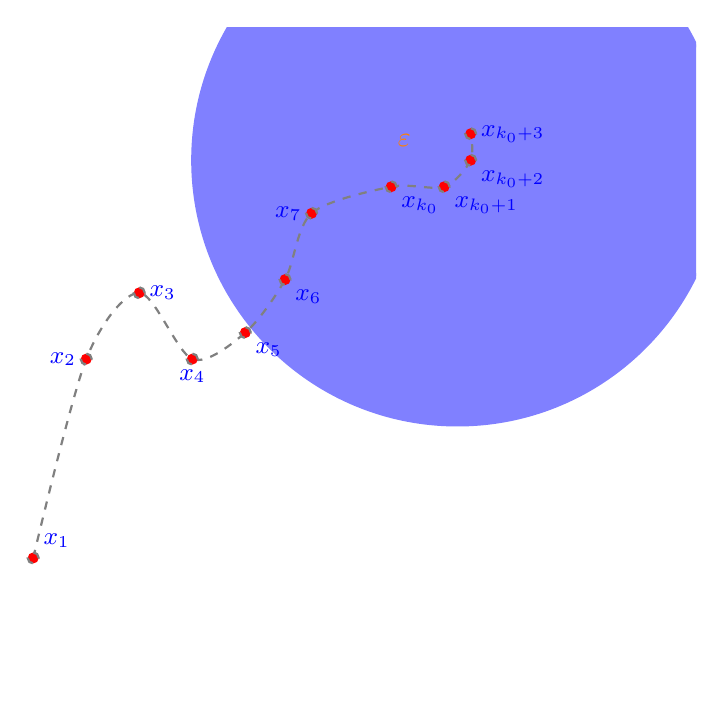
\begin{tikzpicture}[scale=1]
			\begin{axis}[
				width=10cm, height=10cm,
				%axis lines=middle,
				axis lines=none,
				xtick=\empty, ytick=\empty,
				axis equal,
				%enlargelimits,
				xmin=0, xmax=5,
				ymin=0, ymax=3,
				thick,
				xlabel={$x$}, ylabel={$y$},
				axis line style={->}
				]
				% circulo
				\draw[blue!50,fill=blue!50, thick] (axis cs:3.2,3) circle[radius=2];
				\draw[blue!50, ->] (axis cs:3.2,3) -- (axis cs:2.5,3.1); %radio
				
				% Punto límite a
				%\addplot[only marks, mark=*, mark options={fill=blue},  nodes near coords={$a$}, point meta=explicit symbolic ] coordinates { (3,3) [a] };
				
				% Bola abierta centrada en a
				\draw[orange, dashed, thick] (axis cs:3.2,3) circle[radius=70];
				\node[orange] at (axis cs:2.8,3.15) { $\varepsilon$};
				
				
				% Puntos de la sucesión fuera de la bola
				%\addplot[only marks, mark=*, mark options={fill=green} ] coordinates { 	(0,0) (0.5, 1.5) (0.9,2) (1.3, 1.5) (1.7,1.7)  (2.1,2.1)   (2.4, 2.6)   };
				
				% Puntos de la sucesión dentro de la bola
				%\addplot[only marks, mark=*,  mark options={fill=green} ] coordinates { 	(2.7,2.8)  (3.1,2.8)  (3.3,3) (3.3,3.2)  };
				\addplot+[smooth, dashed, gray, mark=*, mark options={fill=red}] coordinates {
					(0,0)        (0.4, 1.5) (0.8,2) (1.2, 1.5) (1.6,1.7) 
					(1.9,2.1)    (2.1, 2.6) (2.7,2.8) (3.1,2.8) (3.3,3) (3.3,3.2)
				};  
				
				% Etiquetas personalizadas
				\node[font=\small\bfseries, text=blue] at (axis cs:0,0)        [above right]  {$x_1$};
				\node[font=\small\bfseries, text=blue] at (axis cs:0.4,1.5)    [left]       {$x_2$};
				\node[font=\small\bfseries, text=blue] at (axis cs:0.8,2)      [  right] {$x_3$};
				\node[font=\small\bfseries, text=blue] at (axis cs:1.2,1.5)    [below]       {$x_4$};
				\node[font=\small\bfseries, text=blue] at (axis cs:1.6,1.7)    [ below right] {$x_5$};
				\node[font=\small\bfseries, text=blue] at (axis cs:1.9,2.1)    [below right]       {$x_6$};
				\node[font=\small\bfseries, text=blue] at (axis cs:2.1,2.6)    [  left]  {$x_7$};
				\node[font=\small\bfseries, text=blue]  at (axis cs:2.7,2.8)    [ below right]  {$x_{k_0}$};
				\node[font=\small\bfseries, text=blue]  at (axis cs:3.1,2.8)    [below right]       {$x_{k_0+1}$};
				\node[font=\small\bfseries, text=blue]  at (axis cs:3.3,3)      [below right]       {$x_{k_0+2}$};
				\node[font=\small\bfseries, text=blue]  at (axis cs:3.3,3.2)    [ right] {$x_{k_0+3}$};
				
				
			\end{axis}
		\end{tikzpicture}  
	\vspace{-6em} % o prueba -2em o -0.5em, según lo que necesites
	
\end{document}